\section{Results}

\subsection{Context and Corpus}

\subsubsection{Saturation}Although \DTLfetch{data}{key}{percentProjectsUsingRegex}{value}\% of the projects observed had at least one regex usage, only \DTLfetch{data}{key}{percentFilesUsingRegex}{value}\% of the files observed had at least one regex usage.

%rather than let datatool construct the table, insert a custom table
%\begin{center}
\begin{tablular}{l|ccccc}
\toprule
source & Q1 & Avg & Med & Q3 & Max \\ 
\midrule
files per project & 2 & 53 & 6 & 21 & 5,963 \\ 
\midrule
files with regex per project & 1 & 11 & 2 & 6 & 541 \\ 
\midrule
regex usages per file & 1 & 2 & 1 & 3 & 207 \\ 
\bottomrule
\end{tabluar}
\end{center}


From the above figure/table, we see that on average each project had \DTLfetch{data}{key}{medRFilePerProj}{value} files containing any regex usage, out of an average of \DTLfetch{data}{key}{medFilePerProj}{value} files.  Each of the files that did have a regex usage had an average of \DTLfetch{data}{key}{medRPerFile}{value} regex usages.  Because we scanned \DTLfetch{data}{key}{nProjScanned}{value} projects, we would expect to have seen \DTLfetch{data}{key}{nExpectedUsages}{value} regex usages, which is lower than the actual \DTLfetch{data}{key}{nUsages}{value} usages observed.

\subsubsection{Regex Functions and Flags}

\begin{figure}[htb]
\centering
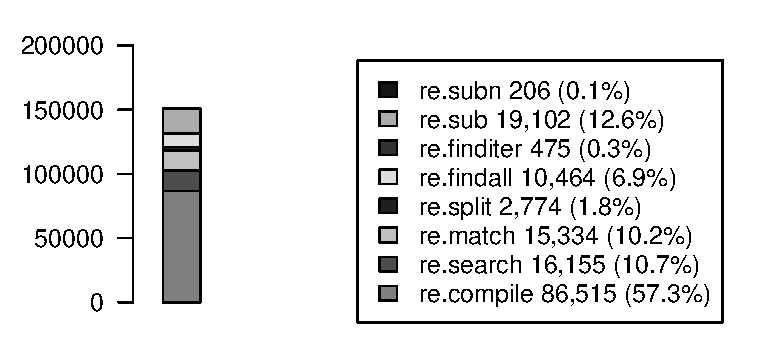
\includegraphics[width=\columnwidth]{../analysis_output/partFunctions.eps}
\caption{How often are the 8 re functions used?}
\label{fig:partFunctions}
\end{figure}

As seen in Figure~\ref{fig:partFunctions} The `compile' function encompasses \DTLfetch{data}{key}{percentCompile}{value}\% of all usages, even though every compiled regex object can only be used by calling other functions.  (TODO-Why?)

\begin{figure}[htb]
\centering
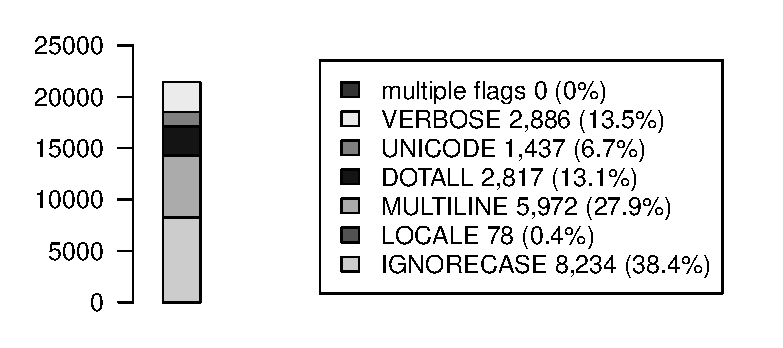
\includegraphics[width=\columnwidth]{../analysis_output/partFlags.eps}
\caption{Which behavioral flags are used?}
\label{fig:digraph}
\end{figure}

\DTLfetch{data}{key}{percentFlags0}{value}\% of all regex usages did not use a flag or specified a non-behavioral flag (default or debug).  Of all behavioral flags used, ignorecase (\DTLfetch{data}{key}{percentI}{value}\%) and multiline (\DTLfetch{data}{key}{percentM}{value}\%) were the most frequently used.  It is also worth noting that although multiple flags can be combined using a bitwise or, this was never observed. (remove this last part if it is observed later)

\subsubsection{{GENERAL CHARACTERISTICS OF REGEXES FOUND}}

...TODO

\subsubsection{{Top 10 Regex Patterns by weight}}


\begin{table}
\begin{center}
\caption{Top 10 Patterns by nProjects (RQ1)}
\label{table:topNW}
\begin{tabular}{lc}
\toprule
pattern & nProjects \\ 
\midrule
\begin{minipage}{2.4in}
\begin{verbatim}
'\x1b\]((?:.|;)*?)(\x07)'\end{verbatim}
\end{minipage}
& 2 \\ 
\midrule
\begin{minipage}{2.4in}
\begin{verbatim}
'\x1b\[\d+m'\end{verbatim}
\end{minipage}
& 1 \\ 
\midrule
\begin{minipage}{2.4in}
\begin{verbatim}
'^[A-Z]'\end{verbatim}
\end{minipage}
& 2 \\ 
\midrule
\begin{minipage}{2.4in}
\begin{verbatim}
'^#format \w*\n'\end{verbatim}
\end{minipage}
& 2 \\ 
\midrule
\begin{minipage}{2.4in}
\begin{verbatim}
'(,\n|[^\n-])+'\end{verbatim}
\end{minipage}
& 1 \\ 
\midrule
\begin{minipage}{2.4in}
\begin{verbatim}
'^[a-df-z]\d*$'\end{verbatim}
\end{minipage}
& 1 \\ 
\midrule
\begin{minipage}{2.4in}
\begin{verbatim}
'[a-zA-Z_:][\w\.\-_:]*\Z'\end{verbatim}
\end{minipage}
& 1 \\ 
\midrule
\begin{minipage}{2.4in}
\begin{verbatim}
'^\?(.*)'\end{verbatim}
\end{minipage}
& 8 \\ 
\midrule
\begin{minipage}{2.4in}
\begin{verbatim}
'Video: \w+'\end{verbatim}
\end{minipage}
& 1 \\ 
\midrule
\begin{minipage}{2.4in}
\begin{verbatim}
'\\.|.'\end{verbatim}
\end{minipage}
& 9 \\ 
\bottomrule
\end{tabular}
\end{center}
\end{table}


\subsubsection{All Features}

Literal tokens were found in (TODO) 101\% of patterns, and accounted for 75\% of all tokens.  Excluding literal tokens and features that were not present in any pattern, the following stats...make a sentence, these are some stats about the features:


\begin{table*}[ht]
\begin{center}
\begin{small}
\caption{How frequently do features appear in projects? (RQ2)}
\label{table:featureStats}
\begin{tabular}
{ll@{ }llc @{ } c @{ }c @{ } c  cccccc @{}}
rank & code & description & example & brics & hampi & Rex & RE2 & nPatterns & \% patterns & nProjects & \% projects \\ 
\toprule[0.16em]
1 & ADD & one-or-more repetition & \begin{minipage}{0.5in}\begin{verbatim}z+\end{verbatim}\end{minipage} & \yes & \yes & \yes & \yes & 5,889 & 44 & 1,197 & 72.8 \\ 
\midrule
2 & CG & a capture group & \begin{minipage}{0.5in}\begin{verbatim}(caught)\end{verbatim}\end{minipage} & \yes & \yes & \yes & \yes & 6,965 & 52.1 & 1,182 & 71.9 \\ 
\midrule
3 & KLE & zero-or-more repetition & \begin{minipage}{0.5in}\begin{verbatim}.*\end{verbatim}\end{minipage} & \yes & \yes & \yes & \yes & 5,882 & 44 & 1,084 & 65.9 \\ 
\midrule
4 & CCC & custom character class & \begin{minipage}{0.5in}\begin{verbatim}[aeiou]\end{verbatim}\end{minipage} & \yes & \yes & \yes & \yes & 4,389 & 32.8 & 1,014 & 61.6 \\ 
\midrule
5 & ANY & any non-newline char & \begin{minipage}{0.5in}\begin{verbatim}.\end{verbatim}\end{minipage} & \yes & \yes & \yes & \yes & 4,537 & 33.9 & 990 & 60.2 \\ 
\midrule
6 & STR & start-of-line & \begin{minipage}{0.5in}\begin{verbatim}^\end{verbatim}\end{minipage} & \no & \yes & \yes & \yes & 3,507 & 26.2 & 836 & 50.8 \\ 
\midrule
7 & RNG & chars within a range & \begin{minipage}{0.5in}\begin{verbatim}[a-z]\end{verbatim}\end{minipage} & \yes & \yes & \yes & \yes & 2,575 & 19.2 & 836 & 50.8 \\ 
\midrule
8 & END & end-of-line & \begin{minipage}{0.5in}\begin{verbatim}$\end{verbatim}\end{minipage} & \no & \yes & \yes & \yes & 3,112 & 23.3 & 816 & 49.6 \\ 
\midrule[0.12em]
9 & NCCC & negated CCC & \begin{minipage}{0.5in}\begin{verbatim}[^qwxf]\end{verbatim}\end{minipage} & \yes & \yes & \yes & \yes & 1,871 & 14 & 765 & 46.5 \\ 
\midrule
10 & WSP & \textbackslash t \textbackslash n \textbackslash r \textbackslash v \textbackslash f or space & \begin{minipage}{0.5in}\begin{verbatim}\s\end{verbatim}\end{minipage} & \no & \yes & \yes & \yes & 2,804 & 21 & 752 & 45.7 \\ 
\midrule
11 & OR & logical or & \begin{minipage}{0.5in}\begin{verbatim}a|b\end{verbatim}\end{minipage} & \yes & \yes & \yes & \yes & 2,068 & 15.5 & 689 & 41.9 \\ 
\midrule
12 & DEC & any of: 0123456789 & \begin{minipage}{0.5in}\begin{verbatim}\d\end{verbatim}\end{minipage} & \no & \yes & \yes & \yes & 2,272 & 17 & 687 & 41.8 \\ 
\midrule
13 & WRD & [a-zA-Z0-9\_] & \begin{minipage}{0.5in}\begin{verbatim}\w\end{verbatim}\end{minipage} & \no & \yes & \yes & \yes & 1,393 & 10.4 & 644 & 39.1 \\ 
\midrule
14 & QST & zero-or-one repetition & \begin{minipage}{0.5in}\begin{verbatim}z?\end{verbatim}\end{minipage} & \yes & \yes & \yes & \yes & 1,836 & 13.7 & 641 & 39 \\ 
\midrule
15 & LZY & as few reps as possible & \begin{minipage}{0.5in}\begin{verbatim}z+?\end{verbatim}\end{minipage} & \no & \yes & \no & \yes & 1,262 & 9.4 & 590 & 35.9 \\ 
\midrule
16 & NCG & group without capturing & \begin{minipage}{0.5in}\begin{verbatim}a(?:b)c\end{verbatim}\end{minipage} & \no & \yes & \no & \yes & 776 & 5.8 & 391 & 23.8 \\ 
\midrule
17 & PNG & named capture group & \begin{minipage}{0.5in}\begin{verbatim}(?P<name>x)\end{verbatim}\end{minipage} & \no & \yes & \no & \yes & 891 & 6.7 & 352 & 21.4 \\ 
\midrule
18 & SNG & exactly n repetition & \begin{minipage}{0.5in}\begin{verbatim}z{8}\end{verbatim}\end{minipage} & \yes & \yes & \yes & \yes & 573 & 4.3 & 335 & 20.4 \\ 
\midrule
19 & NWSP & any non-whitespace & \begin{minipage}{0.5in}\begin{verbatim}\S\end{verbatim}\end{minipage} & \no & \yes & \yes & \yes & 476 & 3.6 & 270 & 16.4 \\ 
\midrule
20 & DBB & $n\le x \le m$ repetition & \begin{minipage}{0.5in}\begin{verbatim}z{3,8}\end{verbatim}\end{minipage} & \yes & \yes & \yes & \yes & 363 & 2.7 & 232 & 14.1 \\ 
\midrule
21 & NLKA & sequence doesn't follow  & \begin{minipage}{0.5in}\begin{verbatim}a(?!yz)\end{verbatim}\end{minipage} & \no & \no & \no & \no & 130 & 1 & 183 & 11.1 \\ 
\midrule
22 & LWB & at least n repetition & \begin{minipage}{0.5in}\begin{verbatim}z{15,}\end{verbatim}\end{minipage} & \yes & \yes & \yes & \yes & 92 & 0.7 & 157 & 9.5 \\ 
\midrule
23 & LKA & matching sequence follows & \begin{minipage}{0.5in}\begin{verbatim}a(?=bc)\end{verbatim}\end{minipage} & \no & \no & \no & \no & 110 & 0.8 & 157 & 9.5 \\ 
\midrule
24 & NWRD & non-word chars & \begin{minipage}{0.5in}\begin{verbatim}\W\end{verbatim}\end{minipage} & \no & \yes & \yes & \yes & 92 & 0.7 & 154 & 9.4 \\ 
\midrule
25 & WNW & word/non-word boundary & \begin{minipage}{0.5in}\begin{verbatim}\b\end{verbatim}\end{minipage} & \no & \no & \no & \yes & 239 & 1.8 & 152 & 9.2 \\ 
\midrule
26 & OPT & options wrapper & \begin{minipage}{0.5in}\begin{verbatim}(?i)CasE\end{verbatim}\end{minipage} & \no & \yes & \no & \yes & 225 & 1.7 & 149 & 9.1 \\ 
\midrule
27 & NLKB & sequence doesn't precede & \begin{minipage}{0.5in}\begin{verbatim}(?<!x)yz\end{verbatim}\end{minipage} & \no & \no & \no & \no & 89 & 0.7 & 132 & 8 \\ 
\midrule[0.12em]
28 & LKB & matching sequence precedes & \begin{minipage}{0.5in}\begin{verbatim}(?<=a)bc\end{verbatim}\end{minipage} & \no & \no & \no & \no & 77 & 0.6 & 118 & 7.2 \\ 
\midrule
29 & ENDZ & absolute end of string & \begin{minipage}{0.5in}\begin{verbatim}\Z\end{verbatim}\end{minipage} & \no & \no & \no & \yes & 89 & 0.7 & 90 & 5.5 \\ 
\midrule
30 & BKR & match the $i^{th}$ CG & \begin{minipage}{0.5in}\begin{verbatim}\1\end{verbatim}\end{minipage} & \no & \no & \no & \no & 59 & 0.4 & 83 & 5 \\ 
\midrule
31 & NDEC & any non-decimal & \begin{minipage}{0.5in}\begin{verbatim}\D\end{verbatim}\end{minipage} & \no & \yes & \yes & \yes & 36 & 0.3 & 57 & 3.5 \\ 
\midrule
32 & BKRN & references PNG & \begin{minipage}{0.5in}\begin{verbatim}\g<name>\end{verbatim}\end{minipage} & \no & \yes & \no & \no & 17 & 0.1 & 28 & 1.7 \\ 
\midrule
33 & VWSP & matches U+000B & \begin{minipage}{0.5in}\begin{verbatim}\v\end{verbatim}\end{minipage} & \no & \no & \yes & \yes & 13 & 0.1 & 15 & 0.9 \\ 
\midrule
34 & NWNW & negated WNW & \begin{minipage}{0.5in}\begin{verbatim}\B\end{verbatim}\end{minipage} & \no & \no & \no & \yes & 4 & 0 & 10 & 0.6 \\ 
\bottomrule[0.13em]
\end{tabular}
\end{small}
\end{center}
\end{table*}


some more text, IDK

\begin{center}
\begin{tabular}{lcc}
\toprule
pair & example from corpus & nTimes \\ 
\midrule
CG::ADD & \begin{minipage}{2in}
\begin{verbatim}
'(:+)'\end{verbatim}
\end{minipage}
& 4189 \\ 
\midrule
CG::KLE & \begin{minipage}{2in}
\begin{verbatim}
'(:)*'\end{verbatim}
\end{minipage}
& 3983 \\ 
\midrule
ANY::KLE & \begin{minipage}{2in}
\begin{verbatim}
'.*'\end{verbatim}
\end{minipage}
& 3709 \\ 
\midrule
CG::ANY & \begin{minipage}{2in}
\begin{verbatim}
'(.)'\end{verbatim}
\end{minipage}
& 3160 \\ 
\midrule
CCC::CG & \begin{minipage}{2in}
\begin{verbatim}
"(['])"\end{verbatim}
\end{minipage}
& 2665 \\ 
\midrule
CCC::ADD & \begin{minipage}{2in}
\begin{verbatim}
'[ ]+'\end{verbatim}
\end{minipage}
& 2612 \\ 
\midrule
RNG::CCC & \begin{minipage}{2in}
\begin{verbatim}
'[A-Z]'\end{verbatim}
\end{minipage}
& 2567 \\ 
\midrule
ADD::KLE & \begin{minipage}{2in}
\begin{verbatim}
'-*(.+)'\end{verbatim}
\end{minipage}
& 2476 \\ 
\midrule
WSP::KLE & \begin{minipage}{2in}
\begin{verbatim}
'\\s*'\end{verbatim}
\end{minipage}
& 2207 \\ 
\midrule
END::STR & \begin{minipage}{2in}
\begin{verbatim}
'^$'\end{verbatim}
\end{minipage}
& 2156 \\ 
\bottomrule
\end{tabular}
\end{center}



OK now that is all for section 2.  Now in section 3 I want to look at clustering by string similarity using mcl clustering algorithm.  Here are the top 6 clusters using various string similarity metrics:

TODO - multiple boxplots for all 5-6 demonstrating cluster size and then also have \# of clusters, pick smallest number of clusters and then use that.




